\section{Treiberentwicklung}
\subsection{Anaylse der Linux Treiber}
Für den verwendeten USB-Video-Grabber sind im Linux Kernel bereits zwei 
verschiedene Treiber vorhanden: 
\begin{itemize}
 \item Das Modul easycap (Kernel Version 2.6.38-3.6)
 \item Die Module stk1160 bzw. saa711x (ab Kernel Version 3.7)
\end{itemize}
Da diese Treiber auf ein im Linux Kern 
vorhandenes größeres Video Framework (V4L2) \autocite{website:v4l2} aufsetzten ist ein direktes Portieren der 
entsprechenden Kernel Module nach RIOT nicht ohne weiteres möglich gewesen.
Trotzdem waren die Linux Kernel Module extrem hilfreich bei der Entwicklung
des RIOT Treibers. Unter anderem konnte anhand dieser Module das zusammenspiel
der beiden Chips und die korrekte Ansteuerung selbiger ermittelt werden.
Insbesondere für den Gateway-Chip \stk{} spielten die Linux Treiber eine
besondere Rolle da für diesen Chip kein Datenblatt verfügbar ist. Die Linux 
Treiber waren somit die einzige, uns verfügbare Dokumentation, für diesen Chip. 

\subsubsection{Analyse auf Quellcode-Ebene}
Da es sich bei dem USB-Video-Grabber um einen Clone des weit verbreiteten
\easycap{} handelt hatten wir zunächst das easycap genannte Kernel
Modul, welches in älteren Linux Versionen vorhanden ist, betrachtet. Dieser Treiber
ist in moderneren Versionen des Linux Kernel (3.7 aufwärts) nicht mehr vorhanden.
Die schlechte Code-Qualität und die nahezu nicht vorhandene Dokumentation dieses Moduls dürfte, unserer Ansicht nach, ein Hauptgrund für dessen Ersetzung durch andere Treiber sein. Wegen der schlechten Lesbarkeit des
Codes war der Informationsgewinn durch das betrachten dieses Codes relativ gering.

In aktuelleren Linux Versionen ist sowohl ein Treiber für den \stk{} (Modulname: stk1160) 
wie auch für den \saa{} (Modulname: saa711x) Chip vorhanden. Diese Treiber sind im wesentlichen 
das Ergebnis eines refactoring des alten easycap Moduls. Der Code dieser Module ist wesentlich 
besser lesbar. Die Dokumentation ist aber auch in diesen Modulen eher mangelhaft. Insbesondere 
lassen sich im Code Kommentare finden die darauf schließen lassen, dass der Autor einige aus easycap übernommenen Teile selber nicht verstanden hat.

Trotz dieser Schwierigkeiten konnten wir anhand der neueren Kernel Module das grundlegende Zusammenspiel der beiden beteiligten Chips nachvollziehen. Einige Unklarheiten sind jedoch erhalten geblieben. Insbesondere wird in den Modulen stk1160 und saa711x Gebrauch von geschachtelten Makros gemacht und nicht dokumentierte magische Zahlen verwendet. 

\subsubsection{Anaylse auf funktionaler Ebene}
Unter Linux gibt es ein Kernel Modul (Modulename: usbmon) welches es erlaubt USB-Datentransfers zu beobachten bzw. 
mitzuschneiden. Als Frontend für dieses Modul kann, dass Netzwerkanalyseprogramm wireshark \autocite{website:wireshark} verwendet werden. 
Jedoch kann usbmon keine Datentransfers beobachten welche DMA (Direct Memory Access) nutzen. Da das stk1160 Modul für den 
asynchronen Datentransfer standardmäßig DMA verwendet waren wir gezwungen das Modul zu modifizieren.
Mit dem modifizierten stk1160, usbmon und wireshark war es uns anschließend möglich den Datentransfer zwischen PC
und USB-Video-Grabber im laufenden Betrieb zu beobachten. 

\subsubsection{Analyseergebnisse}
Durch die Analyse der Linux Module, sowohl auf Quelltextebene wie auch auf funktionaler Ebene, erschloss sich uns das in \autoref{section:zusammenspiel} dargestellte Zusammenspiel der beiden Chips. Des weiteren wurde klar, wie die Initialisierung, der Datentransfer, die Deinitialisierung des
USB-Video-Grabbers und die Kommunikation mit dem \saa{} funktioniert:

\paragraph{Kommunikation mit \saa{}:} Der \saa{} Chip kann von PC-Seite aus nur indirekt über den \stk{} Chip angesteuert werden.
Der \stk{} Chip kann angewiesen werden eine \iic{} Nachricht an den \saa{} Chip zu schicken indem der Inhalt der Nachricht in ein
spezielles Register geschrieben wird. Anschließend muss eine Reihe anderer Register mit speziellen Werten beschrieben werden um
die Nachricht abzuschicken. Wird eine Antwort vom \saa{} Chip erwartet so muss zusätzlich ein Register auf den \stk{} regelmäßig überprüft werden.

\paragraph{Initialisierung:}
\begin{enumerate}
 \item (\saa{} Chip über \iic{}) Der gewünschte Videostandard und andere Timing Parameter werden konfiguriert.
 \item (\saa{} Chip über \iic{}) Der \saa{} wird angewiesen Videodaten an den \stk{} weiterzuleiten.
 \item (\stk{} Chip) Der Chip wird angewiesen isochrone USB-Anfragen zu beantworten.
\end{enumerate}

\paragraph{Datentransfer:} Ist die Initialisierung abgeschlossen können vom PC isochrone USB Pakete an den USB-Video-Grabber
geschickt werden. Jedoch ist darauf zu achten, dass auf dem Host-Controller genügend Bandbreite für den Datentransfer reserviert wird
(Vgl. \emph{Alternate Setting in \autocite{standard:usb2}}). Im wesentlichen funktioniert der Datentransfer wie folgt:
\begin{enumerate}
 \item Leere Pakete (URBs) werden von dem PC an den \stk{} geschickt.
 \item Der \stk{} befüllt diese Pakete mit den Videodaten und sendet diese nach einer unbekannten Zeitspanne zurück an den Sender.
 \item Der Treiber hat einen asynchronen handler welcher beim eintreffen eines Antwortpaketes folgendermaßen agiert:
 \begin{enumerate}
  \item Die Integrität der Daten wird geprüft (anhand einer CRC16 Prüfsumme).
  \item Die Daten werden in einen Puffer geschrieben.
  \item Ein leeres Paket wird erzeugt und an den \stk{} geschickt. 
 \end{enumerate}
\end{enumerate}

\paragraph{Deinitialisierung:}
\begin{enumerate}
 \item (\stk{} Chip) Weiterleiten von Daten, durch setzten von entsprechenden Registerwerten, stoppen.
 \item (\saa{} Chip über \iic{}) Streaming von Videodaten beenden.
 \item Puffer verwerfen, handler für die isochronen URBs beenden und reservierte Bandbreite auf dem Host-Controller wieder freigeben.
\end{enumerate}

\paragraph{}
Die Fehlerbehandlung haben wir im Sinne der Übersichtlichkeit nicht dargestellt.


\subsection{Aufbau und Funktionsweise des RIOT Treibers}
\subsubsection{Aufbau}
Der Quellcode von RIOT \autocite{website:riotosgithub} ist in zwei verschieden git repositories aufgeteilt. Im 
\riotrepo{} ist der Plattformunabhängige Teil des Treibers zu finden. Im \boardsrepo{} hingegen ist der Plattformabhängige Teil enthalten. Darüber hinaus gibt es noch das \projectsrepo{} welches Test- und Demonstrationsprojekte enthält.

In \autoref{fig:srcoverviewriot} ist eine Liste der Dateien zu sehen, welche den Plattformunabhängigen Teil des Treibers bilden.\footnote{wobei RIOT/sys/auto\_init/auto\_init.c nicht Teil des Treibers ist sondern nur modifiziert wurde.} Ziel des Projektes war es einen Treiber für den native port von RIOT zu entwickeln. Daher ist der native port die einzige Plattform welche den Hardwareabhängigen Teil des Treibers enthält. In \autoref{fig:srcoverviewboards} sind die Treiberdateien des native port abgebildet. Die in \autoref{fig:srcoverviewprojects} aufgelisteten Dateien sind Teil eines Demonstrationsprojekt welches die Benutzung des stk1160 Treibers veranschaulichen soll. 

Da der native Port auf einem Host-Betriebsystem (z.B. Linux) läuft wird, mithilfe der Biblothek \libusb{} \autocite{website:libusbx}, der USB Stack des Host-Systems an den native port durchgereicht. Dieser Umstand ist in der Liste der Dateien (\autoref{fig:srcoverviewboards}) nicht sichtbar. Einen ausführlicheren Überblick über die Abhängigkeiten des Treibers bietet daher \autoref{fig:dependsgraph}.

\newgeometry{top=0.5cm,bottom=1.5cm}
\begin{landscape}
\begin{figure}[htbp]
  \centering
  \begin{minipage}[b]{9cm}
  \begin{verbatim}
|-- RIOT
|   |-- core
|   |   |-- include
|   |       \-- usb.h
|   |-- drivers
|   |   |-- stk1160
|   |   |   |-- Makefile
|   |   |   |-- saa711x_regs.h
|   |   |   |-- stk1160.c
|   |   |   |-- stk1160.h
|   |   |   \-- stk1160-reg.h
|   |   \-- include
|   |       |-- stk1160_arch.h
|   |       \-- stk1160.h
|   \-- sys
|       |-- auto_init
|           \-- auto_init.c
    \end{verbatim}
 
    \caption{Liste der Dateien des Treibers im \riotrepo \newline(Plattformunabhängiger Teil)}
    \label{fig:srcoverviewriot}
  \end{minipage}
  \begin{minipage}[b]{9cm}
    \begin{verbatim}
|-- boards
|   |
|   |
|   |
|   |
|   |
|   |
|   |
|   |
|   |
|   |
|   |
|   |
|   \-- native
|       |-- drivers
|       |   \-- native-stk1160.c
|       \-- Makefile
    \end{verbatim}
    \caption{Liste der Dateien des Treibers im \boardsrepo \newline(Plattformunabhängiger Teil)}
    \label{fig:srcoverviewboards}
  \end{minipage}
  \begin{minipage}[b]{9cm}
    \begin{verbatim}
|-- projects
|   |
|   |
|   |
|   |
|   |
|   |
|   |
|   |
|   |
|   |
|   |
|   |
|   |
|   \-- stk1160-test
|       |-- main.c
|       \-- Makefile
    \end{verbatim}
    \caption{List der Dateien\newline im \projectsrepo \newline(Demonstrationsprojekt)}
    \label{fig:srcoverviewprojects}
  \end{minipage}
  \end{figure}
\end{landscape}
\restoregeometry

\begin{figure}[htbp]
 \centering
 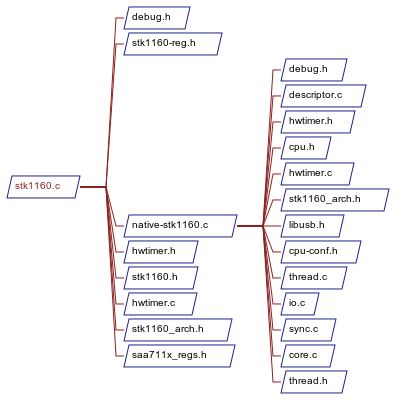
\includegraphics{./DependsOnGraph-stk1160-c.png}
 % DependsOnGraph-stk1160-c.png: 406x400 pixel, 72dpi, 14.32x14.11 cm, bb=0 0 406 400
 \caption{Abhängigkeitsgraph des entwickelten Treibers für RIOT. Die Dateien descriptor.c, libusb.h, io.c, sync.c und core.c sind Teil von \libusb{}.}
 \label{fig:dependsgraph}
\end{figure}

\subsubsection{Funktionsweise}
Die API des Treibers umfasst fünf Funktionen:

\paragraph{stk1160\_init:}
Von einem Benutzer des Treibers wird zunächst die stk1160\_init Funktion aufgerufen. Diese wiederum führt, gemäß der Konventionen in RIOT, die den Build Einstellungen entsprechenden plattformabhängige Initialisierungsfunktion aus. In dem entwickelten Treiber kann es sich hierbei nur um stk1160\_arch\_init in native-stk1160.c handeln.
Diese Funktion initialisiert \libusb{}, sucht nach dem USB-Video-Grabber und reserviert im Erfolgsfall das entsprechende USB-Inteface für den native port.

\paragraph{stk1160\_set\_videosource:} 
Nach der Initialisierung des Treibers sollte festgelegt werden welcher Video-Eingang des USB-Video-Grabbers verwendet wird. 

\paragraph{stk1160\_start\_streaming:}
Sofern die Initialisierung des Treibers erfolgreich war kann anschließend stk1160\_start\_streaming aufgerufen werden. \\ stk1160\_start\_streaming initialisiert sowohl den \stk{} wie auch den \saa{} Chip und startet den isochronen Datenempfang. Als Argument bekommt diese Funktion, eine durch den Treiberbenutzer definierte, handler Funktion übergeben. 
Diese handler Funktion wird von dem Treiber jedes mal aufgerufen wenn neue Videodaten verfügbar sind. Als Argument erhält die handler Funktion ein pointer auf die Videodaten und deren Länge in Bytes.

\paragraph{stk1160\_write\_reg und stk1160\_write\_reg:}
Die Initialisierung des \stk{} Chips erfolgt direkt über das setzten von Registerwerten mithilfe der Funktion stk1160\_write\_reg. Der \saa{} Chip hingegen muss durch eine \iic{} Nachricht gestartet werden. Diese Nachricht wird mit der Funktion stk1160\_i2c\_busy\_wait dem \saa{} Chip übermittelt. Wobei zu beachten ist, dass diese Funktion die Nachricht nicht direkt übermittelt. Stattdessen wird das weiterleiten der Nachricht mithilfe der Funktionen stk1160\_write\_reg und stk1160\_read\_reg an den \stk{} Chip delegiert. 

\paragraph{}
Die Registerwerte werden mit der Funktion usb\_control\_msg gesendet (bzw. empfangen). Der bei der Beschreibung von stk1160\_start\_streaming erwähnte isochrone Datentransfer wird mit init\_iso\_transfer initialisiert. Diese Funktion startet auch einen handling thread mithilfe der Funktion libusb\_event\_handling\_thread. Dieser Thread hat zur Aufgabe den Inhalt von empfangenen isochronen Datenpaketen (die Videodaten) an einem vom Treiberbenutzer übergebenen handler weiterzuleiten und ein neues isochrones Paket an den \stk{} Chip zu schicken. 

\paragraph{}
Der Graph in \autoref{fig:riotcallgraph} illustriert grob die Abfolge der Aufrufe in den verschieden Dateien des Treibers. Ein kommentiertes Beispielprogramm welches die korrekte Verwendung der API des entwickelten Treibers demonstriert ist im \projectsrepo{} zu finden. Zusätzlich sei an dieser Stelle auf die doxygen Dokumentation verweisen. Diese Dokumentation lässt sich in \emph{RIOT/doc/doxygen} mit einem Aufruf von \emph{make} generieren und anschließend als man page oder in html betrachten.
\newgeometry{left=0.1cm,right=0.1cm}
\begin{figure}[htbp]
 \centering
 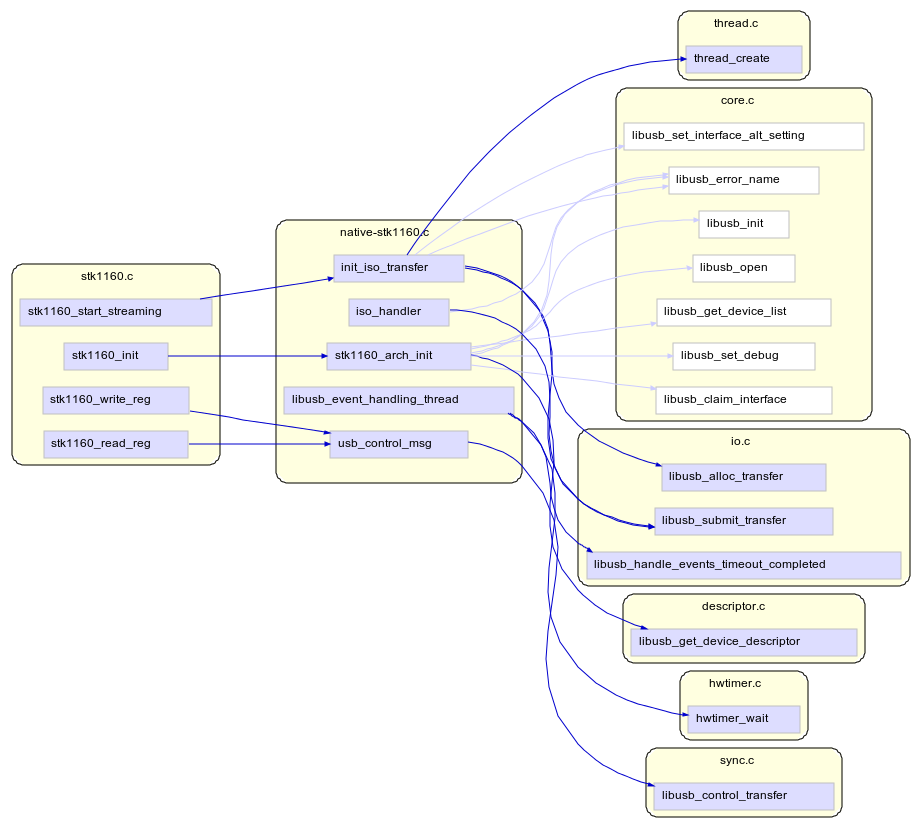
\includegraphics[scale=0.63]{./ClusterCallButterflyGraph-native-stk1160-c-highlighted.png}
 % ClusterCallButterflyGraph-native-stk1160-c-highlighted.png: 922x830 pixel, 72dpi, 32.53x29.28 cm, bb=0 0 922 830
 \caption{Callgraph des entwickelten RIOT Treibers. core.c, io.c, descriptor.c und sync.c sind Teil von \libusb{}. Zwecks Übersichtlichkeit sind die Kanten nach Funktionen in core.c ausgegraut. In stk1160.c sind alle Funktionen, bis auf stk1160\_set\_videosource, aufgelistet welche Teil der API des Treibers sind.}
 \label{fig:riotcallgraph}
\end{figure}
\restoregeometry
\subsection{Vorgehen bei der Implementierung}
Der Treiber wurde inkrementell im Pair-Programming erarbeitet. Jedes Teilentwicklungsziel des Treibers setzte sich im wesentlichen aus vier Phasen zusammen:
\begin{enumerate}
 \item Analyse des entsprechenden Teiles des Linux Treibers durch Quelltexteinsicht, Debug-Ausgaben und betrachten des Datenverkehrs (usbmon und wireshark)
 \item Implementierung des Features im RIOT Treiber
 \item Debuggen des geschriebenen Codes
 \item Vergleich des Datenverkehrs des RIOT Treibers mit dem des Linux Treibers
\end{enumerate}

Wobei zu erwähnen ist, dass eine Reihe von Tools die Entwicklung erheblich vereinfacht haben:
\begin{itemize}
 \item git: ein VCS welches auch von dem RIOT Team verwendet wird. 
 \item ctags und cscope: Erlauben die schnelle Navigation in umfangreichen C-Quellcode.
 \item gdb: Da der native port ein auf dem Host-System ausführbares Binary ist (unter Linux ein ELF) lassen sich Fehler mit dem GNU Debugger nachvollziehen.
 \item usbmon und wireshark: Mit diesen Werkzeugen lässt sich der Datenverkehr auf dem USB-Bus relativ komfortabel beobachten. Ohne diese beiden Tools wäre die Entwicklung des Treibers noch zeitaufwändiger gewesen. 
\end{itemize}

\subsection{Probleme und Herausforderungen}
Die Probleme bei der Entwicklung ergaben sich Hauptsächlich aus dem Fehlen des Datenblattes für den \stk{} Chip wie auch der mangelhaften Dokumentation der Linux Treiber. Daher war die größte Herausforderung bei der Entwicklung des Treibers für RIOT die genaue Funktionsweise des USB-Video-Grabbers zu ermitteln. Wobei das ermitteln der Funktionsweise durch, oftmals sehr langwierige, Analyse- / Debug- Sessions erreicht werden konnte.

Ein weiteres Problem ist der Fakt, dass RIOT zum Zeitpunkt der Entwicklung dieses Treibers keinen USB Stack enthielt. Dieses Problem konnten wir jedoch umgehen indem der Treiber lediglich für den native port und \libusb{} entwickelt wurde. Somit kann der USB-Stack des Host-Systems verwendet werden. Es ist jedoch Anzumerken, dass der Treiber auch im Hinblick auf einen eventuell später verfügbaren RIOT USB-Stack geschrieben wurde.  